\documentclass[a4paper,12pt]{article}


%%% Работа с русским языком
\usepackage{cmap}					% поиск в PDF
\usepackage{mathtext} 				% русские буквы в формулах
\usepackage[T2A]{fontenc}			% кодировка
\usepackage[utf8]{inputenc}			% кодировка исходного текста
\usepackage[english,russian]{babel}	% локализация и переносы
\usepackage{indentfirst}
\frenchspacing

\newcommand{\vyp}{\ensuremath{\hookrightarrow}}
\renewcommand{\epsilon}{\ensuremath{\varepsilon}}
\renewcommand{\phi}{\ensuremath{\varphi}}
\renewcommand{\kappa}{\ensuremath{\varkappa}}
\renewcommand{\le}{\ensuremath{\leqslant}}
\renewcommand{\leq}{\ensuremath{\leqslant}}
\renewcommand{\ge}{\ensuremath{\geqslant}}
\renewcommand{\geq}{\ensuremath{\geqslant}}
\renewcommand{\emptyset}{\varnothing}
\newcommand{\Ra}{\ensuremath{\Rightarrow}}
\newcommand{\ra}{\ensuremath{\rightarrow}}
\newcommand{\LRa}{\ensuremath{\Leftrightarrow}}
\newcommand{\tbf}{\textbf}
\newcommand{\ov}{\ensuremath{\overline}}
\newcommand{\CC}{\ensuremath{\mathbb{C}}}
\newcommand{\RR}{\ensuremath{\mathbb{R}}}
\newcommand{\NN}{\ensuremath{\mathbb{N}}}
\newcommand{\QQ}{\ensuremath{\mathbb{Q}}}
\newcommand{\ZZ}{\ensuremath{\mathbb{Z}}}

%%% Дополнительная работа с математикой
\usepackage{amsmath,amsfonts,amssymb,amsthm,mathtools} % AMS
\usepackage{icomma} % "Умная" запятая: $0,2$ --- число, $0, 2$ --- перечисление

%% Номера формул
%\mathtoolsset{showonlyrefs=true} % Показывать номера только у тех формул, на которые есть \eqref{} в тексте.
%\usepackage{leqno} % Нумереация формул слева

%% Свои команды
\DeclareMathOperator{\sgn}{\mathop{sgn}}

%% Перенос знаков в формулах (по Львовскому)
\newcommand*{\hm}[1]{#1\nobreak\discretionary{}
{\hbox{$\mathsurround=0pt #1$}}{}}



%%% Работа с картинками
\usepackage{graphicx}  % Для вставки рисунков
\graphicspath{{images/}{images2/}}  % папки с картинками
\setlength\fboxsep{3pt} % Отступ рамки \fbox{} от рисунка
\setlength\fboxrule{1pt} % Толщина линий рамки \fbox{}
\usepackage{wrapfig} % Обтекание рисунков текстом

%%% Работа с таблицами
\usepackage{array,tabularx,tabulary,booktabs} % Дополнительная работа с таблицами
\usepackage{longtable}  % Длинные таблицы
\usepackage{multirow} % Слияние строк в таблице

%%% Теоремы
\theoremstyle{plain} % Это стиль по умолчанию, его можно не переопределять.
\newtheorem{theorem}{Теорема}[section]
\newtheorem{proposition}[theorem]{Утверждение}
 
\theoremstyle{definition} % "Определение"
\newtheorem{corollary}{Следствие}[theorem]
\newtheorem{problem}{Задача}[section]
 
\theoremstyle{remark} % "Примечание"
\newtheorem*{nonum}{Решение}

%%% Программирование
\usepackage{etoolbox} % логические операторы

%%% Страница
\usepackage{extsizes} % Возможность сделать 14-й шрифт
\usepackage{geometry} % Простой способ задавать поля
	\geometry{top=20mm}
	\geometry{bottom=20mm}
	\geometry{left=5mm}
	\geometry{right=15mm}
 %
\usepackage{fancyhdr} % Колонтитулы
 	\pagestyle{fancy}
 	\renewcommand{\headrulewidth}{1pt}  % Толщина линейки, отчеркивающей верхний колонтитул
%\fancypagestyle{firstpage}{
	\rhead{\large{Исыпов Илья}}
%}
% 	\lfoot{Нижний левый}
% 	\rfoot{\large{Рябых Владислав, Б05-905}}
% 	\rhead{Верхний правый]}
% 	\chead{Верхний в центре}
 	\lhead{\large{Рябых Владислав}}
%	\cfoot{Нижний в центре} % По умолчанию здесь номер страницы

\usepackage{setspace} % Интерлиньяж
\onehalfspacing % Интерлиньяж 1.5
%\doublespacing % Интерлиньяж 2
%\singlespacing % Интерлиньяж 1

\usepackage{lastpage} % Узнать, сколько всего страниц в документе.

\usepackage{soul} % Модификаторы начертания

\usepackage{hyperref}
\usepackage[usenames,dvipsnames,svgnames,table,rgb]{xcolor}
\hypersetup{				% Гиперссылки
    unicode=true,           % русские буквы в раздела PDF
    pdftitle={Заголовок},   % Заголовок
    pdfauthor={Автор},      % Автор
    pdfsubject={Тема},      % Тема
    pdfcreator={Создатель}, % Создатель
    pdfproducer={Производитель}, % Производитель
    pdfkeywords={keyword1} {key2} {key3}, % Ключевые слова
    colorlinks=true,       	% false: ссылки в рамках; true: цветные ссылки
    linkcolor=red,          % внутренние ссылки
    citecolor=black,        % на библиографию
    filecolor=magenta,      % на файлы
    urlcolor=cyan           % на URL
}

\usepackage{csquotes} % Еще инструменты для ссылок

%\usepackage[style=authoryear,maxcitenames=2,backend=biber,sorting=nty]{biblatex}

\usepackage{multicol} % Несколько колонок

\usepackage{tikz} % Работа с графикой
\usepackage{pgfplots}
\usepackage{pgfplotstable}

\usepackage{caption}
\long\def\comment{}
\setlength{\abovecaptionskip}{7pt}
\setlength{\belowcaptionskip}{7pt}
\mathtoolsset{showonlyrefs}
\newcommand{\RNumCaps}[1]
{\MakeUppercase{\romannumeral #1}}

\begin{document}

\begin{titlepage}
	\begin{center}
		
		\textsc{\LARGE Московский\\[-0.2cm]Физико-Технический Институт\\[0.1cm]\large (национальный исследовательский университет)}\\[1.5cm] 
		
	
\includegraphics[width=0.3\textwidth]{hv_s_no_bg.png}~\\[1cm]

	\textsc{\Large Оптика. \\ Лабораторный практикум. }\\[0.2cm]

	% Title
	\HRule \\[0.4cm]
	{ \LARGE \bfseries Лабораторная работа № 4.1.1 \\ Изучение центрированных оптических систем. \\[0.4cm] }

	\HRule \\[1.5cm]
		
		% Author and supervisor
		\noindent
		\begin{minipage}{0.4\textwidth}
			\begin{flushleft} \large
			\end{flushleft}
		\end{minipage}%
		\begin{minipage}{0.4\textwidth}
			\begin{flushright} \large
			\end{flushright}
		\end{minipage}
		
		
		\large{\begin{flushright}
				\vfill
				\textbf{Выполнили}:\\
				\textbf{Рябых Владислав,\\}
				\textbf{Исыпов Илья\\}
				\textbf{группа Б05-905}
		\end{flushright}}
		
		
		{\large \today}\\
		
		
	\end{center}
\end{titlepage}

\subsubsection*{Цель работы:} изучить методы определения фокусных расстояний линз и сложных оптических систем; определить характеристики оптической системы, составленной из тонких линз; изучить недостатки реальных линз — сферическую и хроматическую аберрации.

\subsubsection*{Оборудование:} оптическая скамья с набором рейтеров, положительные и отрицательные линзы, экран, осветитель с ирисовой диафрагмой, зрительная труба, светофильтры, кольцевые диафрагмы, линейка.

\section*{Теория}

Измерение фокусного расстояния по методу Аббе основано на определении поперечного увеличения для нескольких  различных положений предмета на оптической оси исследуемой системы. На рис. 1 представлена соответствующая схема эксперимента.
\begin{center}
	\begin{figure}[bhtp!]
		\centering
	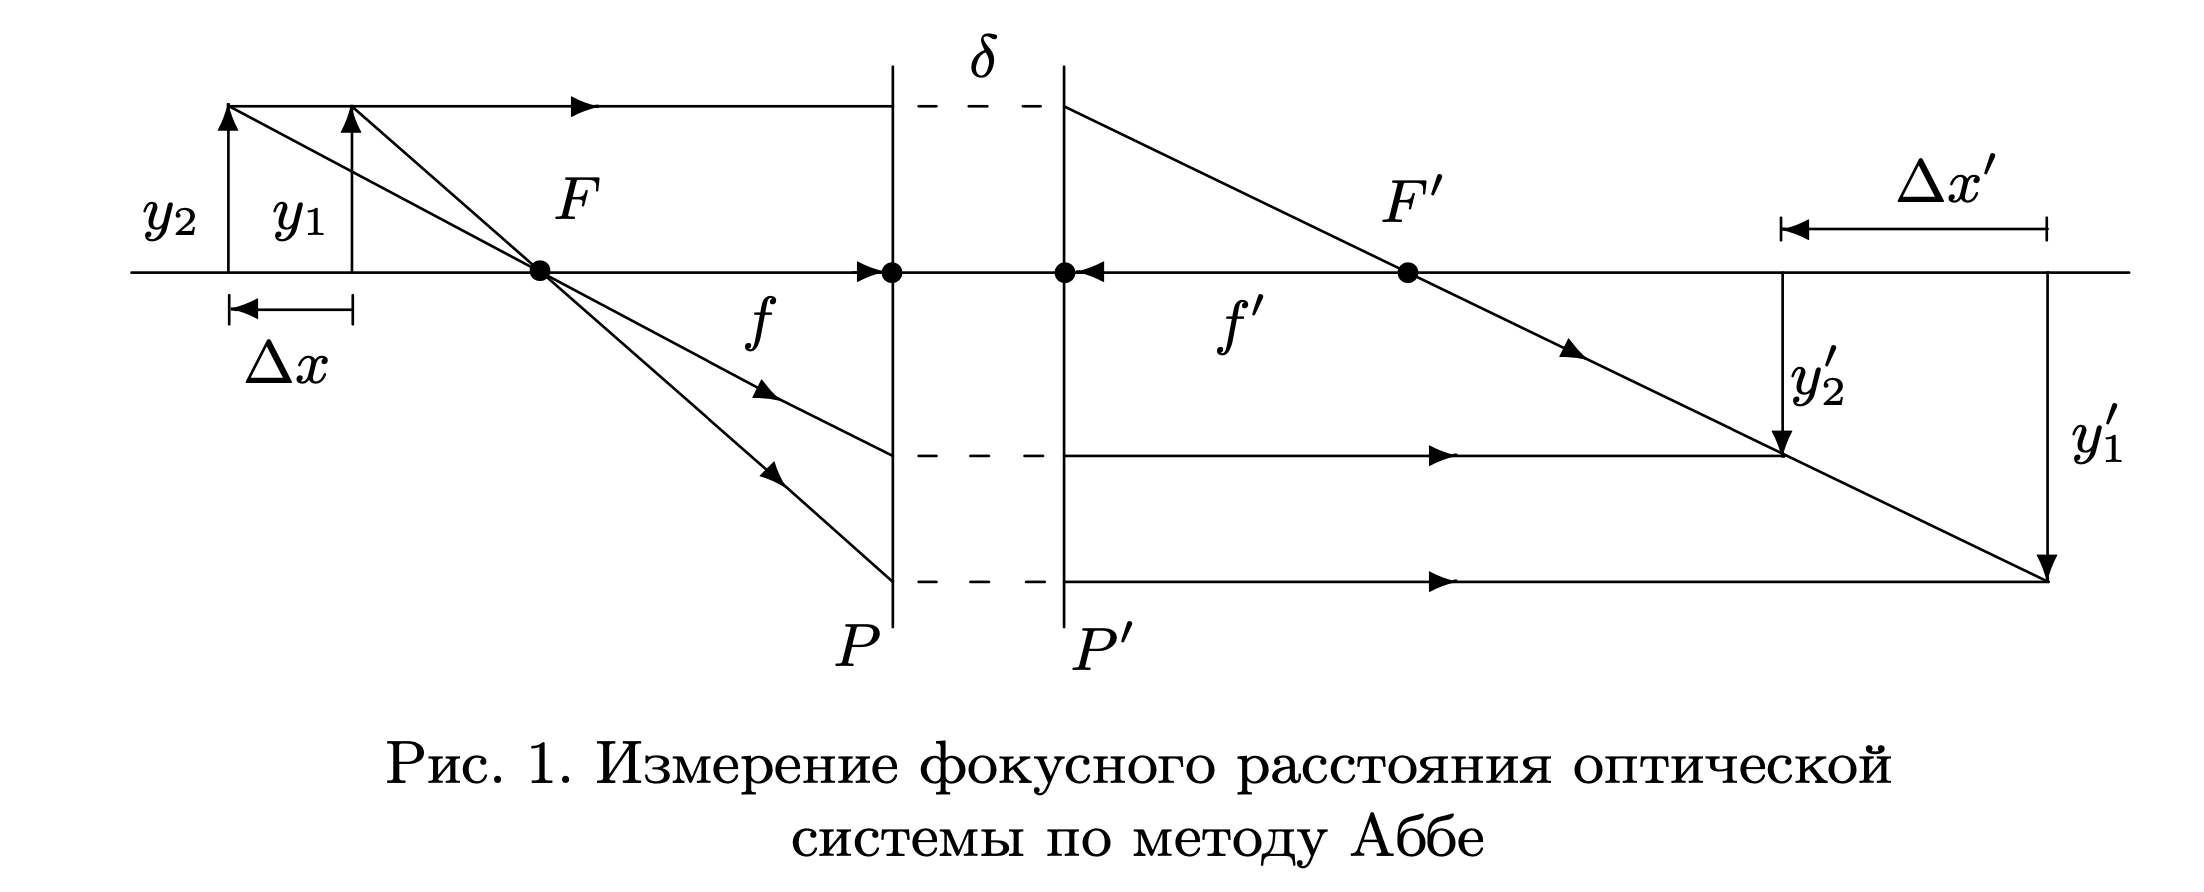
\includegraphics[width=16cm]{1.1.1.png}
	\end{figure}
\end{center}
Пусть $\Delta x =x_2 - x_1$ --- смещение объекта,  $\Delta x' = x_2' - x_1'$ --- смещение изображения. $\Delta\left(\frac{y'}{y}\right) = \frac{y_2'}{y_2} - \frac{y_1'}{y_1}$ ---  приращение поперечного увеличения. $\Delta\left(\frac{y}{y'}\right) = 1/\Delta\left(\frac{y'}{y}\right)$.  Тогда 
фокусное расстояние системы можно выразить через положения предмета и соответствующие увеличения по формуле: \begin{equation}\label{formula1}
	f = \frac{\Delta x}{\Delta\left(\frac{y}{y'}\right)} = -\frac{\Delta x'}{\Delta\left(\frac{y'}{y}\right)}
\end{equation}

\begin{center}
	\begin{figure}[bhtp!]
		\centering
	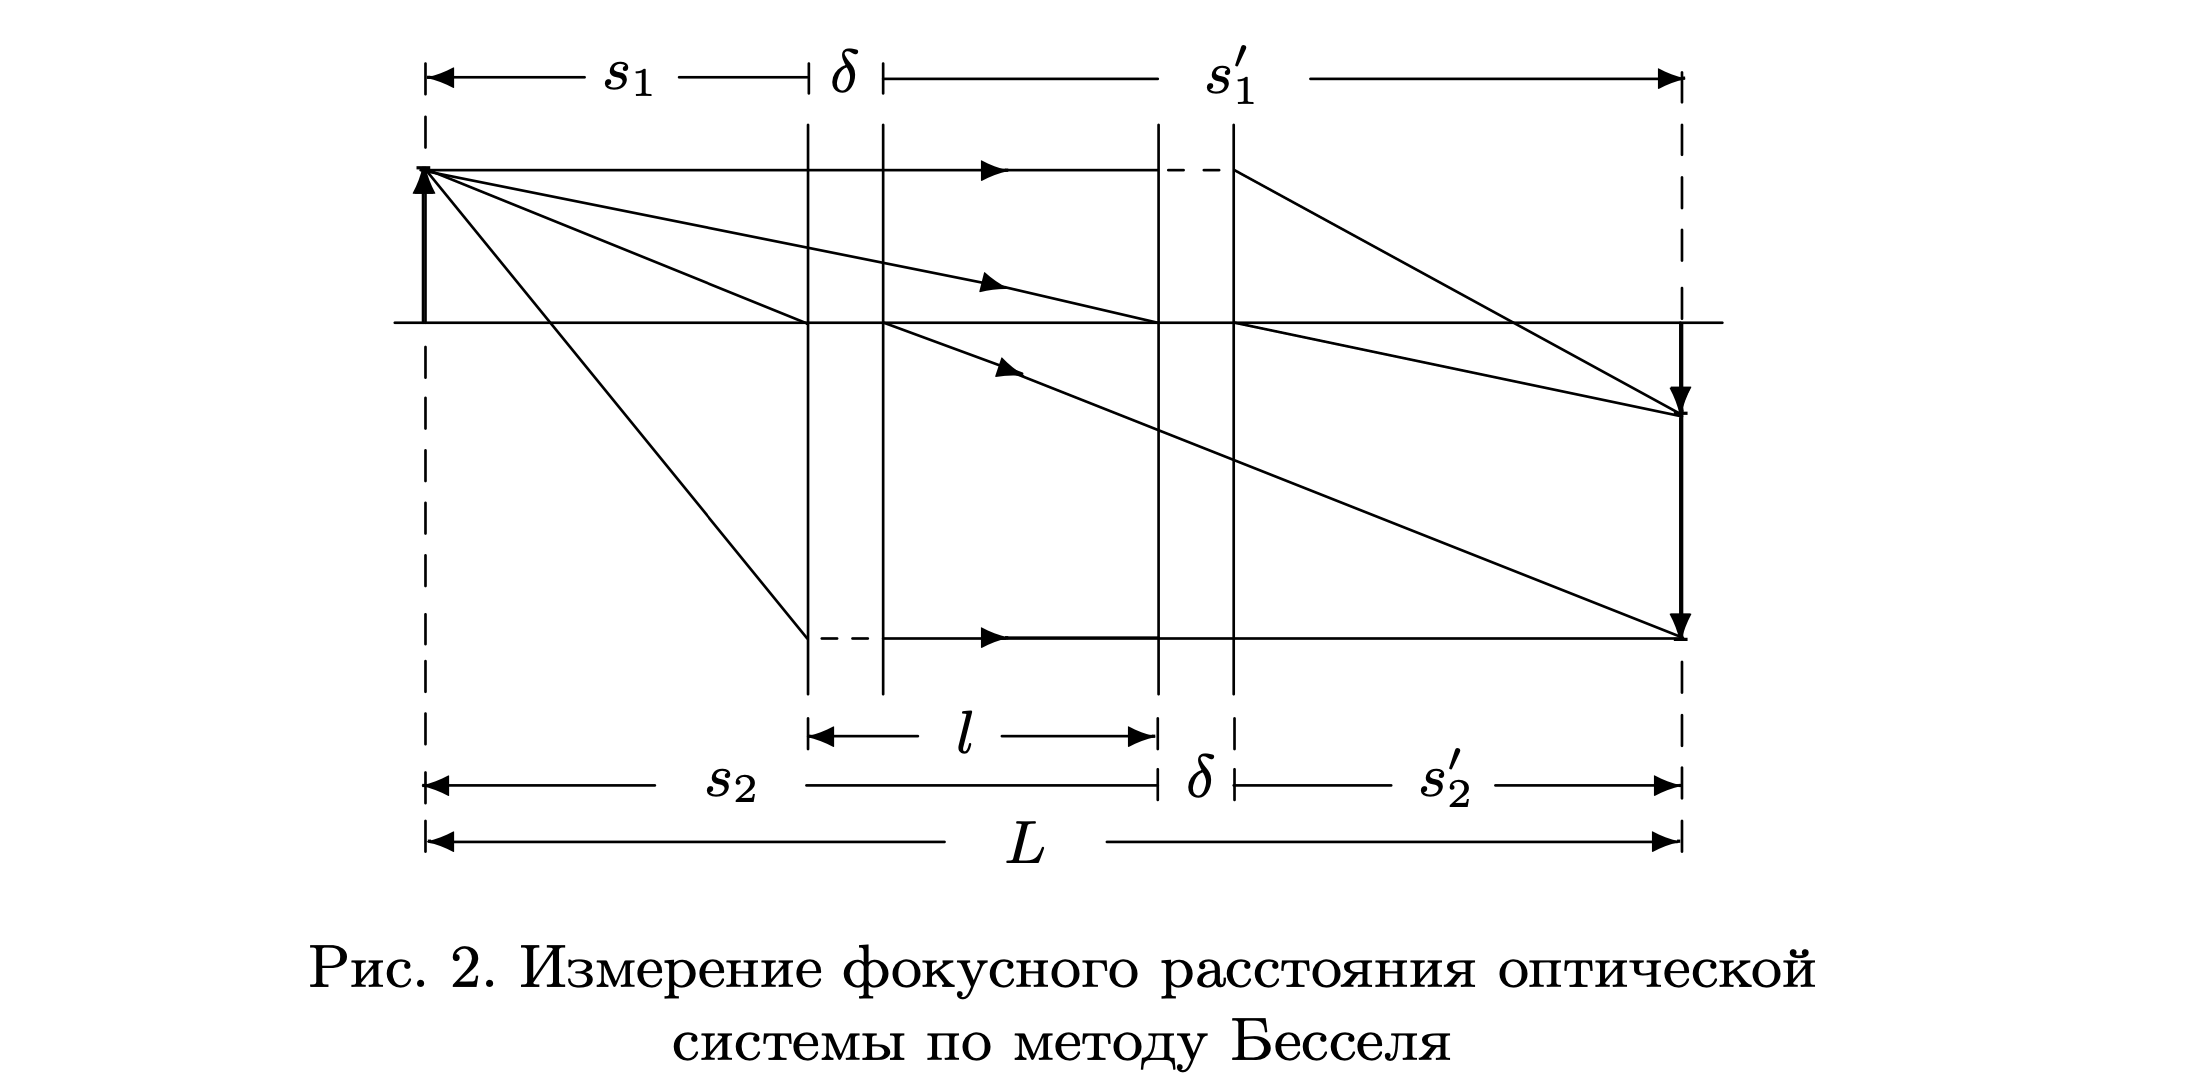
\includegraphics[width=15cm]{1.1.2.png}
	\end{figure}
\end{center}
С целью уменьшения случайной ошибки, возникающей при фокусировке изображения, измерения следует проводить несколько раз, усредняя полученные данные.

Схема метода Бесселя для случая, когда $n = n'$ и $f' = -f$, представлена на рис. 2. Она основана на том, что при заданном расстоянии L между предметом  и экраном мы имеем квадратное уравнение относительно расстояния $s$ от главной плоскости пространства предметов до предмета ($s < 0$) которое выражается формулой :
\begin{equation}\label{formula2}
	\frac{1}{f} = -\frac{1}{s} + \frac{1}{\delta - L +s}
\end{equation}
имеющее при  $L > 4f +\delta$ два решения. С учётом симметрии и направлений расстояний, положения предметов определяются соотношениями $s'_2 = -s_1\,,\,s'_1 = -s_2$. Для расстояния $L$ между предметом и экраном и расстояния $l$ между двумя положениями системы (линзы) получаем, что  $L-\delta = s'_1 - s_1$ , $l = s_1 + s_1' = s_1 -s_2$. Поэтому справедливы следующие выражения:
\begin{equation}\label{formula3}
	\begin{cases}
		s_1 = -\frac{1}{2}(L - \delta - l) \\
		s'_1 = \frac{1}{2}(L - \delta + l) \\
	\end{cases}
\end{equation}
Подставляя \eqref{formula3} в формулу (1.22), после несложных преобразований находим выражение: 
\begin{equation}\label{formula4}
	f = \frac{(L-\delta)^2 - l^2}{4(L-\delta)}
\end{equation}
При $|\delta| \ll L$  Получаем рабочую формулу : 
\begin{equation}\label{formula5}
	f = \frac{L^2- l^2}{4L}
\end{equation}
Если выполнить измерения для двух пар величин $L$ и $l$, то из двух уравнений вида  \eqref{formula4} можно найти обе характеристики системы: $f$ и $\delta$.
\newline\newline


\subsubsection*{Два основных метода определения фокусного расстояния тонкой собирающей линзы.}
\begin{enumerate}
	\item[\textbf{\RNumCaps{1}}] 
	Пусть $a$ и $a'$ — расстояния до предмета и его изображения от плоскости линзы, причём $a < 0$, $a' > 0$, если предмет находится слева, а его изображение — справа от линзы; Тогда фокусное расстояние $f > 0$ легко находится из уравнения тонкой линзы:
	\begin{equation}\label{formula6}
	-\frac{1}{a} + \frac{1}{a'} = \frac{1}{f}
	\end{equation}
	Для измерения фокусного расстояния достаточно провести измерения по стандартной схеме «предмет — линза — экран» при произвольном расстоянии между предметом и экраном с различными значениями $a$.
	\item[\textbf{\RNumCaps{2}}] Фокусное расстояние тонкой собирающей линзы можно определить с помощью зрительной трубы, настроенной на бесконечность. Разместив между предметом и зрительной трубой положительную линзу и перемещая её вдоль оси системы, можно найти резкое изображение предмета в окуляре зрительной трубы. При этом расстояние от середины линзы до предмета равно фокусному расстоянию тонкой линзы.
\end{enumerate}

\subsubsection*{Способы Определения фокусного расстояния тонкой рассеивающей линзы.}
\begin{center}
	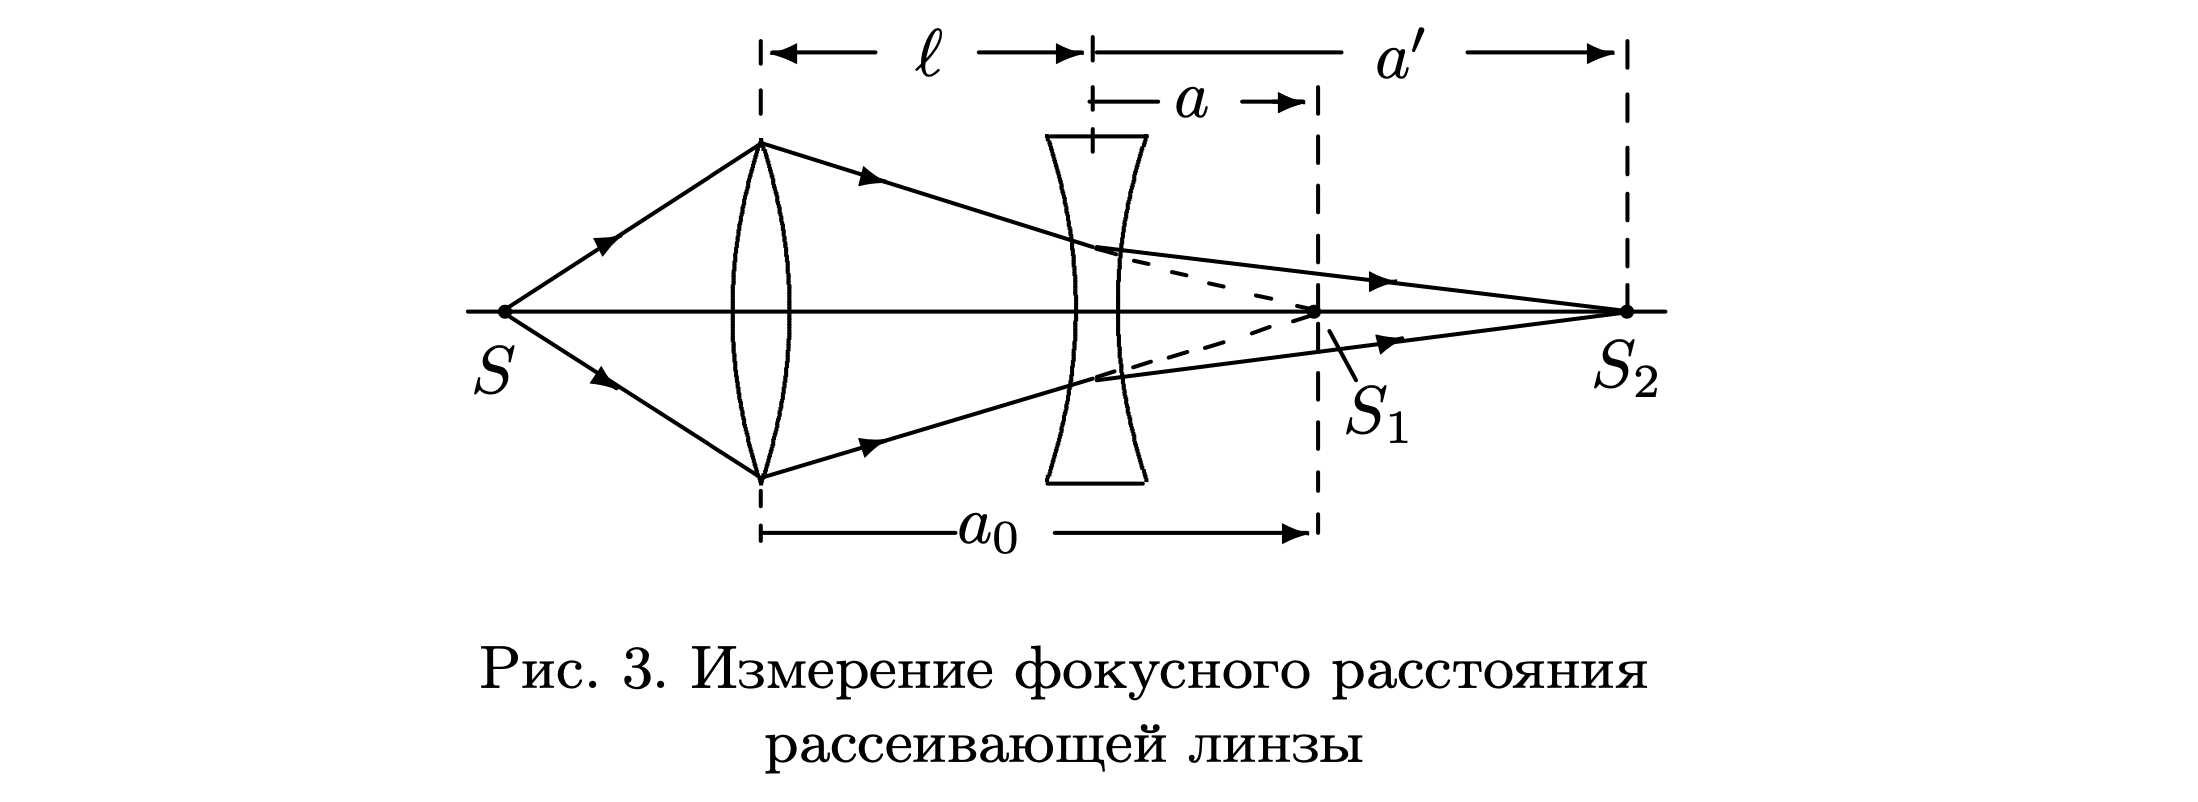
\includegraphics[width=14cm]{1.1.3.png}
\end{center}
\begin{enumerate}
	\item[\textbf{\RNumCaps{1}}] 
	Сначала с помощью собирающей линзы получают на экране действительное изображение предмета $S$ (точка $S_1$ на рис. 3). Затем на пути  выходящих лучей располагают исследуемую рассеивающую линзу и, отодвигая экран, получают чёткое изображение предмета на экране, образованное двумя линзами. Точка $S_1$ пересечения сходящихся лучей играет по отношению к рассеивающей линзе роль мнимого источника. Изображение источника переместится теперь в точку $S_2$.Определив расстояния $a = a_0 - l > 0$ и $a' > 0$, рассчитывают фокусное расстояние рассеивающей линзы по формуле \eqref{formula6}.
	\item[\textbf{\RNumCaps{2}}] Если расстояние a на рис.3 совпадает с модулем фокусного расстояния рассеивающей линзы, то изображение $S_2$ перемещается в бесконечность. Параллельность пучка можно установить с помощью зрительной трубы. Зная расстояние от первой линзы до точки $S_1$ и расстояние между линзами, нетрудно определить фокусное расстояние тонкой рассеивающей линзы. 
\end{enumerate}


\subsubsection*{Определение положения главных и фокальных плоскостей  оптической системы.}
Для нахождения главных плоскостей системы недостаточно знать фокусное расстояние, нужно определить ещё положения главных фокусов. Это можно сделать при помощи зрительной трубы, настроенной на бесконечность. Отложив от главных фокусов отрезки, равные фокусному расстоянию, можно найти положения главных плоскостей системы. При этом необходимо учитывать возможность различного взаимного расположения кардинальных точек (плоскостей) сложной системы.
Все характеристики оптической системы, состоящей из двух тонких линз, можно рассчитать по фокусным расстояниям $f_1$, $f_2$ каждой линзы и оптическому интервалу $\Delta$ или расстоянию между центрами линз $l_{12}$.


\section*{Ход работы}


Введём следующие обозначения для типов линз:

\begin{itemize}
	\item $+$ собирающая линза;
	\item $-$ рассеивающая линза;
\end{itemize}

Для начала определим какие из линз являются собирающими, а какие рассеивающими. Для этого в темной комнате откроем окно и поднесём к противоположной стене линзу. Также можно замерить линейкой приблизительное фокусное расстояние таких линз. Занесём данные в таблицу \ref{tab:1}.     
\begin{table} [bhtp!] 
	\centering
	\begin{tabular}{|c|c|c|}\hline
		номер & тип линзы & фокусное расстояние, см      \\\hline
		1           & $+$   & $11.5\pm 0.1$                    \\\hline
		2           & $+$  & $13\pm 0.1$                       \\\hline
		3           & $+$   & $11\pm 0.1$                       \\\hline
		4           & $-$   & не установлено                       \\\hline
		
	\end{tabular}
	\caption{определение типа линз}
	\label{tab:1}
\end{table}

Для Центровки линз  достаточно перемещать их вдоль осей, добиваясь чёткого изображения и совпадения центра экрана и изображения объекта.

\subsubsection*{Измерение фокусного расстояния методом Бесселя}
Для линз $1-3$ проведём серии экспериментов методом Бесселя -- снимем необходимые расстояния и по формуле \eqref{formula6} (с учётом знаков) найдём $f$. Данные занесем в таблицу \ref{tab:2}. Чтобы вычислить $f$ для линзы $4$, будем использовать ее вместе с собирающей линзой $3$. Результаты запишем в таблицу \ref{tab:3}
\begin{table} [!hbp] 
	\centering
	\begin{tabular}{|c|c|c|c|c|} \hline
		& предмет-линза, см & линза-изобр,см & предмет-изобр, см& $f$, см  \\\hline
		\multirow{4}{*}{линза 1}    & $35.5\pm0.1$ & $20.5\pm0.1$  & $56.0\pm0.1$& $13.0\pm 0.4$                             \\\cline{2-5}
		& $20.5\pm0.1$ & $35.5\pm0.1$  & $56.0\pm0.1$& $13.0\pm 0.4$  \\\cline{2-5}
		& $17.2\pm0.1$ & $52.8\pm0.1$  & $70.0\pm0.1$& $13.0\pm0.4$  \\\cline{2-5}
		& $53.0\pm0.1$ & $17.0\pm0.1$  & $70.0\pm0.1$& $12.9\pm0.4$  \\\hline
		\multirow{4}{*}{линза 2}        & $55.0\pm0.1$& $20.0\pm0.1$& $75.0\pm0.1$& $14.7\pm 0.4$                                    \\\cline{2-5}
		& $20.5\pm0.1$& $54.6\pm0.1$& $75.1\pm0.1$& $14.9\pm 0.4$            \\\cline{2-5}
		& $71.4\pm0.1$& $18.6\pm0.1$& $90.0\pm0.1$& $14.8\pm 0.4$           \\\cline{2-5}
		& $18.9\pm0.1$& $71.1\pm0.1$& $90.0\pm0.1$& $14.9\pm 0.4$           \\\hline
		\multirow{4}{*}{линза 3}       & $26.1\pm0.1$& $23.9\pm0.1$& $50.0\pm0.1$& $12.5\pm 0.4$                                    \\\cline{2-5}
		& $23.5\pm0.1$& $26.5\pm0.1$& $50.0\pm0.1$& $12.5\pm 0.4$            \\\cline{2-5}
		& $15.6\pm0.1$& $59.5\pm0.1$& $75.1\pm0.1$& $12.4\pm 0.4$            \\\cline{2-5}
		& $59.0\pm0.1$& $16.0\pm0.1$& $75.0\pm0.1$& $12.6\pm 0.4$          \\\hline
		
	\end{tabular}
	\caption{метод Бесселя для положительных линз}
	\label{tab:2}
\end{table}


\begin{table} [bhtp!] 
	
	\centering
	\begin{tabular}{|c|c|c|c|}
		\hline
		3 линза - экран(без 4 линзы), см & между линзами,см & 4 линза-изобр, см&   $f$,см\\\hline
		$26.4\pm0.1$ & $17.6\pm 0.1$&$42.4\pm 0.1$ & $-10.7\pm 0.3$ \\\hline
	\end{tabular}
	\caption{метод Бесселя для отрицательной линзы}
	\label{tab:3}
\end{table}


\subsubsection*{Определение с помощью зрительной трубы}
Для определения $f$ с помощью трубы необходимо настроить ее на бесконечность. Для этого идем в коридор, смотрим в дальнее окно и добиваемся чёткого изображения. После этого ставим собирающую линзу на расстоянии от предмета, примерно равном фокусному. На небольшом расстоянии от линзы помещаем и центрируем  трубу. Передвигая линзу,  получаем в окуляре  чёткое изображение. Расстояние предмет-линза и будет фокусным. Далее повернем линзу и проделаем эксперимент снова. Опыт необходимо проделать для линз 1,2. Для надежности, проделаем независимо этот опыт дважды. Занесем данные в таблицу \ref{tab:4}.

\begin{table}  [bhtp!]
	\centering
	\begin{tabular}{|c|c|c|}
		\hline
		линза & $f$ до разворота, см &$f$ после разворота, см
		\\\hline
		1& $13.5\pm0.1$& $12.5\pm0.1$ 
		\\\hline
		2& $15.0\pm0.1$& $16.0\pm0.1$ 
		\\\hline
		1& $13.6\pm0.1$& $12.8\pm0.1$ 
		\\\hline
		2& $14.7\pm0.1$&$16.0\pm0.1$
		\\\hline
	\end{tabular}
	\caption{определение фокусного расстояния с помощью зрительной трубы}
	\label{tab:4}
\end{table}

По результатам видно, что фокусы линз расположены не симметрично, поэтому линзы нельзя считать идеальными.

Для измерения $f$ рассеивающей линзы воспользуемся схемой, показанной на рисунке 3. Сначала получаем на экране увеличенное изображение предмета при помощи положительной линзы, замеряя расстояние до экрана $a_0$. Далее ставим сразу за экраном трубу, настроенную на бесконечность, а вместо экрана исследуемую рассеивающую линзу, перемещением которой добиваемся чёткого изображения в окуляре. Фокусное расстояние рассеивающей линзы будет равно $l-a_0$, $l$ - расстояние между линзами. Повторим эксперимент после разворота линзы.  Получили 
$f_1 = - 11\pm0.1$ см и $f_2 = -9\pm0.1$ см соответственно.


\subsubsection*{Определение фокусного расстояния и положения главных и фокальных плоскостей системы.}
Для определения фокусного расстояния системы с линзами 1 и 2 по методу Аббе (рис. 1) поместим экран на дальнем конце скамьи, и, перемещая источник света, получаем резкое изображение на экране. $x'$- расстояние от предмета до первой линзы, $y_1'$- размер изображения(исходный объект -- стрелка длиною 2 см). Далее перемещаем экран и фиксируем новое изображение, а также его размер $y_2'$. Расстояние между линзами $ 5.1\pm0,1$ см.
Измерив все необходимые данные, воспользуемся формулой \eqref{formula1} и занесём результаты в Таблицы \ref{tab:5} и \ref{tab:6}.
\begin{table}[bhtp!]
	\centering
	\begin{tabular}{|c|c|c|c|c|c|}\hline
		$\Delta x$, см&   $\Delta x'$, см &  $y'$, см& $y''$, см & $f_{\Sigma_1}$, см & $f_{\Sigma_2}$, см \\\hline
		$4.0\pm 0.1$& $41 \pm 0.1$ & $34\pm0.1$& $14.9\pm 0.1$& $8.8 \pm0.1$ & $7.2\pm 0.1$  \\ \hline
	\end{tabular}
	\caption{Метод Аббе, порядок линз $(1,2)$}
	\label{tab:5}
\end{table}



\begin{table}[bhtp!]
	\centering
	\begin{tabular}{|c|c|c|c|c|c|}\hline
		$\Delta x$, см&   $\Delta x'$, см &  $y'$, см& $y''$, см & $f_{\Sigma_1}$, см & $f_{\Sigma_2}$, см \\\hline
		$4.5\pm 0.1$& $14.7 \pm 0.1$ & $2.4\pm0.1$& $6.6\pm 0.1$& $8.5 \pm0.1$ & $7.0\pm 0.1$  \\ \hline
	\end{tabular}
	\caption{Метод Аббе, порядок линз $(2,1)$}
	\label{tab:6}
\end{table}

Для нахождения положения главных фокусов системы необходимо закрепить  трубу за второй линзой и,
медленно отодвигая осветитель от системы,  получить резкое изображение предмета в окуляре. Для определения  положение главного фокуса системы  следует измерить расстояние от этой линзы до предмета. Получаем: $x = 3.5\pm 0.1$ см, $F_{\Sigma_1} =6.6 \pm 0.1$ см, $F_{\Sigma_2} = 6.1\pm 0.1$ см.
Построим на миллиметровке:
\begin{center}
	\begin{figure}[bhtp!]
		\centering
		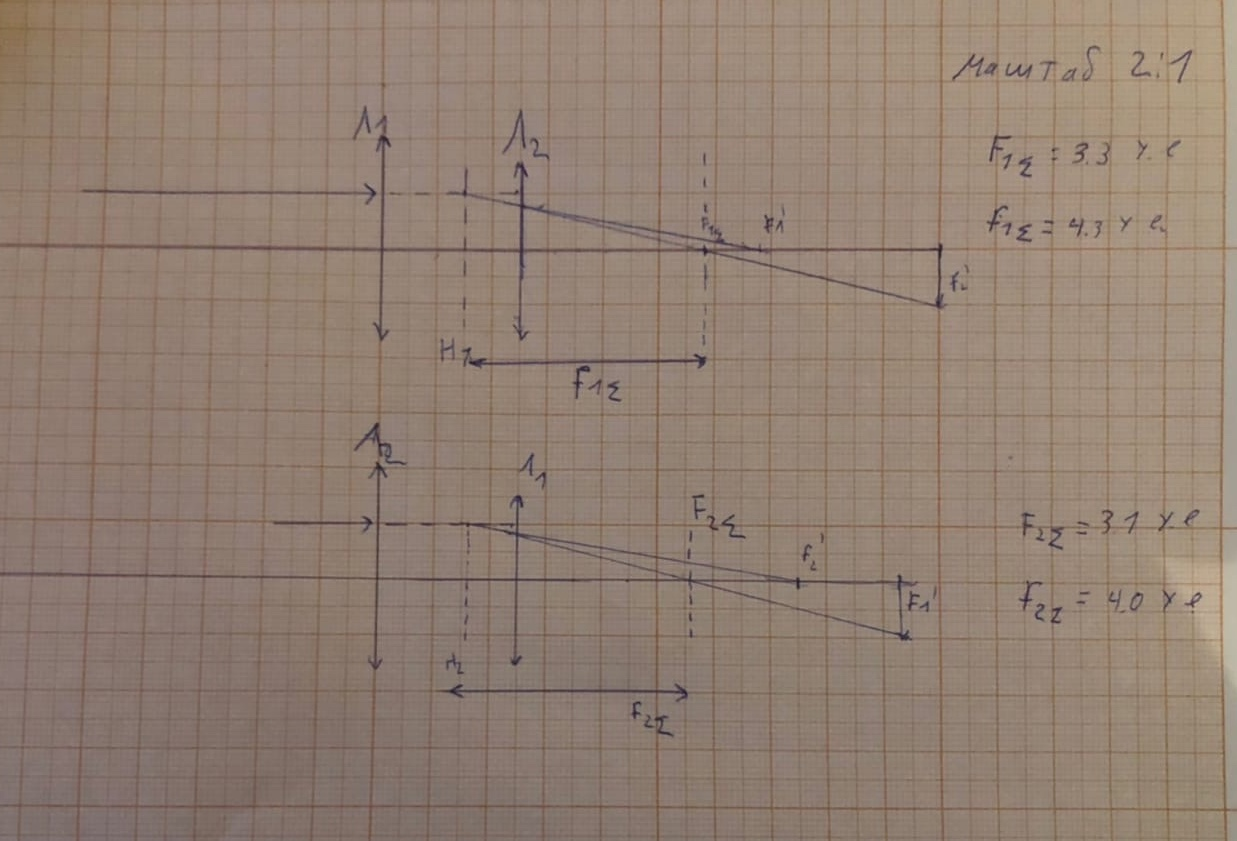
\includegraphics[width=14 cm]{kD3aQ9ZTqlE.jpg}
	\end{figure}
\end{center}
Получили: $f_{\Sigma_1}=8.6\pm0.2$ см, $f_{\Sigma_2}=8.0\pm0.2$ см.  В одном из случаев результат совпадает с полученным выше с точностью до ошибки, а во втором нет, хотя и значения лежат довольно близко.


\subsection*{Основные типы Аберраций}


 \subsubsection*{Сферические аберрации} Для качественного наблюдения сферической аберрации необходимо расположить источник и экран на дальних концах скамьи. Далее нужно установить линзу $3$, способную перемещаться относительно рейтера в продольном направлении, на расстоянии $a_1$, чуть большем фокусного. Надев на линзу диафрагму диаметром $2h = 1$ см, нужно получить на удалённом экране резкое изображение диафрагмы осветителя. После чего, заменив диафрагму на диаметром $2h = 4$ см, убеждаемся, что $a_2$ значительно отличается от $a_1$.
 
	Для получения количественных значений, воспользуемся трубой вместо экрана, а также нониусной шкалой. Постепенно заменяя диафрагмы и регулируя расстояние с помощью нониусного винта, снимем зависимость $\Delta S(h)$, $\Delta S$ -- смещение от фокусного расстояния при $2h=1$ см и занесём данные в таблицу 7:
	
	\begin{table}[h] 
		\centering
		\begin{tabular}{|c|c|}
			\hline
			$\Delta S$, м $\cdot10^{-4}$ &$h$, см \\ \hline
			$0$         &$0.5$ \\ \hline
			$110 \pm 1$          & $1.0$ \\ \hline
			$240 \pm 1$      &   $2.0$ \\ \hline
		\end{tabular}
		\caption{Сферические аберрации}
	\end{table}
	По данным в таблице чётко видно, что при изменении радиуса диафрагмы изменяется и фокус, что и является сферической аберрацией.
	
\subsubsection*{Хроматические аберрации.} С помощью трех светофильтров, нониусного винта, а также линзы номер три можно пронаблюдать хроматические аберрации. Для этого, надевая поочередно светофильтры, следим за изменением фокусного расстояния. Результаты приведены в таблице \ref{tab:8}.
	
	\begin{table} [bhtp!]
		\centering
		\begin{tabular}{|c|c|} \hline
			светофильтр& $\Delta S$, см \\\hline 
			желтый & $-0.53 \pm 0.1$ \\\hline
			красный& $0.64\pm 0.1$\\\hline
			голубой &  $-1.12\pm 0.1$ \\ \hline
		\end{tabular}
		\caption{Хроматические аберрации}
		\label{tab:8}
	\end{table}

	Используя эти данные, посчитаем число Аббе($D,C,F$- желтый, красный и голубой соответственно):
	\begin{equation*}
	\nu = \frac{f_D}{f_C -f_F} \thickapprox 64.5 \pm 0.1
	\end{equation*}

Ошибка оценена из соображений, что погрешность определения нуля была $\pm 0.05$ см



\section*{Вывод}
При изучении сложных оптических систем мы пришли к выводу, что линзы не являются идеальными. При изучении аберраций наблюдалась зависимость фокусного расстояния от длины волны, а также от радиуса диафрагмы, что подтверждает наличие аберраций. 


\end{document}